\documentclass[12pt]{article}
\usepackage{indentfirst}
\usepackage[margin=1in]{geometry}
\usepackage{hyperref}
\usepackage{pgfplots}
\usepackage{float}
\usepackage{amsmath}

\title{Math IA Rough Draft}
\author{hyg172}
\date{May 2020}

\begin{document}
\maketitle

\tableofcontents
\newpage

\section{Exploration}
IDEA 1
T-test

Does the FIDE rating of the top 100 US chess players have a correlation with their USCF ratings?

The null hypothesis is there is no correlation between FIDE rating and USCF rating.

Top 100 US Chess players as of October: (USCF)
\url{http://www.uschess.org/component/option,com_top_players/Itemid,371?op=list&month=1910&f=usa&l=R:Top%20Overall.&h=Overall}

FIDE ratings are located:
\url{https://ratings.fide.com/top_lists.phtml}

IDEA 2
How does the US Top 10 players compare with 10 other countries top 10?
ANOVA

The null hypothesis is that there is not a significant difference in mean rating among the 10 countries.

FIDE ratings can be found at 
\url{https://ratings.fide.com/top_lists.phtml}

\subsection{Introduction}
As a young child, I've always been interested in the idea of quantifying and relating objects using numbers. This was initially a usefool tool in visualizing basic arithmetic. When I started playing tournament chess, I recieved a chess rating, or a number used to quantify one's chess strength relative to others. There are multiple such systems that give chess player ratings, for example online chess websites such as Lichess and Chess.com have their own rating systems, and even countries have their own rating systems. However, the governing body of chess, FIDE, has their own rating system that allows a standard rating for comparison between countries with otherwise different rating systems. This led to the foci of the investigation on how FIDE ratings compare to USCF ratings with respect to the top 10 players in the US and also comparing the strengths of the top 10 players of the top 10 countries.
\subsection{Research Questions}
How do the FIDE ratings compare to USCF ratings of the top 10 chess players in the US?

How different are the ratings between the top 10 players of the top 10 chess country federations?
\subsection{Hypothesis}
I predict that USCF ratings will be not much different from FIDE ratings. However, USCF ratings may be slightly higher as the overall pool of players with FIDE ratings has stronger players.

I predict that there will be a statistically significant difference between the FIDE ratings of the top 10 players of the top 10 countries as they have different concentrations of strong players. 

\section{Analysis}
\subsection{Data}
\subsubsection{USCF vs FIDE}
Suprisingly, the top 10 players by USCF rating differ from FIDE's list of the top 10 US players by FIDE rating. This difference is due to the fact that FIDE and USCF tournaments have different criteria for a tournament to be valid. Due to this, we will find the respective USCF ratings of the top 10 US players by FIDE rating. Nevertheless, the top players American players by FIDE and USCF rating are the same, just in different order.

\begin{center}
\begin{tabular}{rr}
FIDE & USCF\\
\hline
2822 & 2894\\
2765 & 2826\\
2758 & 2834\\
2736 & 2836\\
2712 & 2787\\
2683 & 2744\\
2677 & 2758\\
2673 & 2749\\
2660 & 2733\\
2659 & 2748\\
\end{tabular}
\end{center}

Additionally, it is important to note that the USCF top player list was accurate as of December 2019 and the FIDE list was accurate as of January 2020. 

\begin{center}
\begin{tabular}{rrrrrrrrrr}
Russia & USA & China & India & Ukraine & Armenia & Azerbaijan & Hungary & France & Poland\\
\hline
2777 & 2822 & 2805 & 2758 & 2698 & 2773 & 2770 & 2758 & 2770 & 2758\\
2774 & 2765 & 2758 & 2721 & 2685 & 2689 & 2765 & 2696 & 2679 & 2725\\
2753 & 2758 & 2732 & 2716 & 2685 & 2663 & 2668 & 2663 & 2651 & 2639\\
2752 & 2736 & 2726 & 2654 & 2678 & 2642 & 2666 & 2649 & 2640 & 2619\\
2747 & 2712 & 2705 & 2648 & 2662 & 2641 & 2659 & 2626 & 2633 & 2614\\
2731 & 2683 & 2683 & 2639 & 2660 & 2641 & 2625 & 2621 & 2625 & 2611\\
2726 & 2677 & 2669 & 2638 & 2650 & 2632 & 2622 & 2620 & 2604 & 2609\\
2723 & 2673 & 2667 & 2637 & 2644 & 2617 & 2609 & 2617 & 2603 & 2603\\
2705 & 2660 & 2664 & 2636 & 2634 & 2613 & 2598 & 2595 & 2600 & 2601\\
2704 & 2659 & 2640 & 2630 & 2631 & 2611 & 2538 & 2593 & 2572 & 2589\\
\end{tabular}
\end{center}

\subsection{Data Processing}
\subsubsection{T-Test}

\begin{center}
\begin{tabular}{rr}
Standard Deviation & Mean\\
\hline
54 & 2715\\
\end{tabular}
\end{center}

\begin{center}
\begin{tabular}{rr}
Standard Deviation & Mean\\
\hline
54 & 2791\\
\end{tabular}
\end{center}


\begin{figure}[H]
\centering
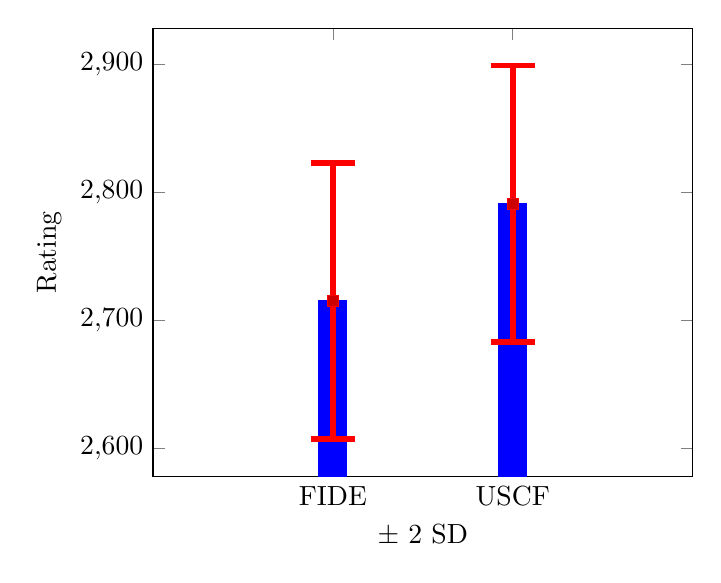
\begin{tikzpicture}
\begin{axis}[
symbolic x coords={FIDE, USCF},
xtick=data,
enlarge x limits = 1,
xlabel = {\(\pm \) 2 SD},
ylabel = {Rating}
]
\addplot+[ybar,fill=blue] coordinates {
(FIDE, 2715)
(USCF, 2791)
};
\addplot+[only marks, error bars/.cd,
y dir=both, y explicit, error bar style={line width=2pt}, error mark options={
rotate=90,
red,
mark size=8pt,
line width=2pt}] 
coordinates {(FIDE, 2715) +-(0,108) (USCF, 2791) +-(0,108)
};
\end{axis}
\end{tikzpicture}
\caption{FIDE and USCF Ratings}
\end{figure}

Null Hypothesis: There is not a significant differece between the mean FIDE rating and the mean USCF rating.

Alternate Hypothesis: There is a significant differrence between the mean FIDE rating and the mean USCF rating. 

Test Statistic: 
% fix t-test equation
\begin{equation}
    t_{(n-1)} \; \textrm{d}f = \dfrac{x}{\dfrac{y}{z}} = -3.16
\end{equation}

p-value: P(t \(\leq\) 0.005)
\subsubsection{ANOVA Test}

Because the p-value is less than 0.05, the null hypothesis cannot be accepted. Therefore, we provisionally accept the alternate hypothsis that there is a significant difference between USCF and FIDE ratings.

\section{Evaluation}
\subsection{Data based answer to the research question}
\subsection{Extensions}
It would also be interesting to look at countries concentration of grandmasters, international masters, as well as titled players as a measure of strength. 

It would also be interesting to see which country's rating system is most similar to FIDE ratings.

Additionally, it would be interesting to see how online ratings compared to FIDE ratings.











\end{document}




